%%%%%%%%%%%%%%%%%%%%%%%%%%
%% Template file for an IEE conference article
%% Trim Size: A4 Paper
%% iiai-conference.tex   :   29-2-08
%% Tex file to use with iiai-c.sty written in Latex2E.
%% The content, structure, format and layout of this style file is the
%% property of International Institute of Applied Informatics
%% Copyright 2013 by International Institute of Applied Informatics
%% All rights are reserved.
%% Created by Satoshi Takahashi, UEC, Japan, Antoine Bossard, AIIT, Japan, Wen Gu, JAIST, Japan and Shun Okuhara, Mie University, Japan
%%%%%%%%%%%%%%%%%%%%%%%%%%
\documentclass[11pt, onecolumn, twoside, a4paper]{article}
\usepackage{iiai-c}
%\usepackage{} % for times new roman; Antoine will send email
\usepackage{graphicx}
\usepackage{amsmath}
\usepackage{amssymb}
\usepackage{amsthm}
\usepackage{lipsum}
\usepackage{mathptmx}

\usepackage[rm,up,sc,topmarks,calcwidth,pagestyles]{titlesec}
\titleformat{\section}{\Large\bfseries\rmfamily}{\thesection}{1em}{}
\titleformat{\subsection}{\large\bfseries\rmfamily}{\thesubsection}{1em}{}
\titleformat{\subsubsection}{\large\it\rmfamily}{\thesubsubsection}{1em}{}

\newtheorem{theorem}{Theorem}
\newtheorem{lemma}[theorem]{Lemma}
\newtheorem{corollary}[theorem]{Corollary}
\newtheorem{property}[theorem]{Property}
\newtheorem{define}[theorem]{Definition}
\newtheorem{assume}[theorem]{Assumption}
\def \Re {\mathbb{R}}


% Edit by IEE editor
\authorshead{S.~Takahashi, A.~Bossard, T.~Matsuo, T.~Fukushima}
\titlehead{IIAI Open Conference Publication Series {\LaTeX} Template}
\vol{1}
\no{1}
\year{2015}
\setcounter{page}{48} % edit
\page{48}
\lastpage{62} % edit


\title{A Platform for Searching Texts for Desired Expressions in a User-editable Pattern Matching Environment for Language Learning}
\author{Tatsuya Katsura \thanks{Graduate School of Environmental, Life, Natural Schience and Technology, Okayama University, Okayama, Japan}, Koichi Takeuchi \thanks{Faculty of Environmental, Life, Natural Science and Technology, Okayama University, Okayama, Japan} }
\date{}
\begin{document} 

\maketitle
\thispagestyle{empty}

\section*{Abstract}
In this paper we propose a platform of pattern matching system that can extract required phrases or sentences in texts.
Finding certain expressions in texts are often needed in language learning, e.g, examples of case markers
between a predicate and an argument, or possible nouns in subject of a verb in a certain meaning. In previous studies,
several types of systems, containing concordancers, are proposed. However, it is not easy to apply combined
patterns because the pattern mathing templates are previously fixed.
% flexibilityが必要 背景としては task specific な systemで作られているので 英語検索に特化はしてると
% 小論文での表現でみんなが同じようにどう使っているかといった表現の分析に利用するのは容易ではない
% その一番の原因は flexibility 
Thus, we propose a flexible phrase searching system in which the users can create search patterns
by combining blocks of basic search templates. % 拡張性がある blockで 提案する
%長すぎる時はここを消す
One of the characteristics the proposed system is that the user can also specify where to be highligted
in texts with the blocks.
To realize the function of combining patterns by the users, the proposed system employs
Prolog as the base of the data structure. The platform of the searching system is implemented
on an Web server with JavaScript-based interface and database system. 
% ブロックにいろいろ設定することで,ユーザは組み合わせてさらに使うことができる
%To realize the pattern matching of predicate-argument structure, 
%the system emplopys several NLP tools.
In the performance test, we shows that the proposed system can deal with relatively large sclale texts
(10,000 sentences), and also demonstrate the combined patterns can be applied to the texts.
In this paper we discuss the system architecture and the extendability of the pattern matching. 
%
%\section*{Keywords}
%About four key words or phrases in alphabetical order, separated by commas.
%
%\noindent
\\[2mm]
{\it Keywords: } Pattern matching, Concordancer, Block-based programming, Prolog


\section{Introduction}
%education
Extraction of some phrases and expressions in texts is considered essential function in langugage education.
For example, case markers located between a predicate and an object in Japanese language are various
rules and alternations\footnote{The verbs {\it morau} (get) and {\it eru} (obtain) are almost the same meaning
but {\it morau} has alternation between the case markers {\it ni/kara} as {\it kare ni/kara morau}
((I) get (it) from him.), and 
{\it eru} can only takes {\it kara} in this meaning as {\it kare kara/*ni eru}.},
% 彼 から もらう,彼に もらう but, 彼から 得る 彼に 得る.
then language learners need to search for examples of predicate-argument
examples in Japanese texts. 
%also, search for similar phrases in student essays. this is eample for use in education. 
As a tool for searching texts, various kinds of concordancer are proposed, however, most concordancers
are targeted for English. From the results of natural language processing study, several dependency parsers for
Japanese are available, thus it is possible to compose a complex text searching system if
the language learners can build NLP tools. But language learners are not NLP or software engineer,
thus, we need an environment to build patterns by searching for phrases or expressions without
needing programming.


when user want to obtain some verb-nouns or predicate preposition,
concodancer is available the basic functions character, word matchina are available,
but more extendede cases are no method. 

, however, more combined search, for example, semantic meaning
of predicate buy-sell and linguitic alternation, kara/wo in Japanese
dependency 

% もらう,得るの質問 native https://ja.hinative.com/questions/17482159





%作ったもの
日本語に対するパターンマッチングシステム



\section{Related Studies}
An IIAI electronic copyright form should accompany your final submission or registration of the conference. The instruction of copyright transfer is announced at the conference webpage. Authors are responsible for obtaining any security clearances for the copyright form submission.


\section{Platfrom of Pattern Matching System}
user editable pattern with visual handling, Construction of pattern is not easy, the
user shoud apply the assumed patterns, see the results and then tune up the patterns.
Thus, editing space and results should be exist.

Patterns are combinations, conbining by basic blocks and extract every where matched.

\include{system_inst}



%\begin{figure}[htbp]
% \begin{center}
%    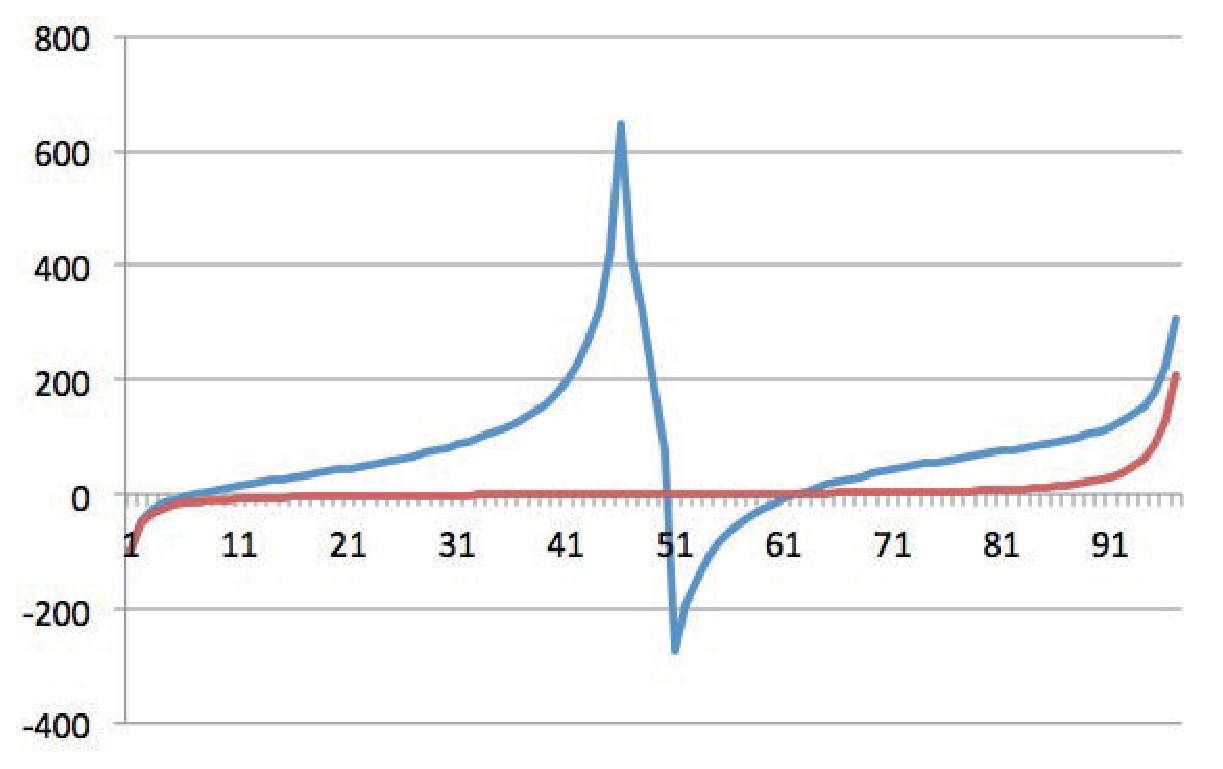
\includegraphics[clip,width=10.0cm]{./fig1.eps}
%    \caption{Example}
%    \label{fig:example}
%  \end{center}
%\end{figure}


\section{References}


\subsection{Example}
\subsubsection{Article in a collection}
\subsubsection{Article in a conference proceedings}
\subsubsection{Article in a journal or magazine}
\subsubsection{Blog}
\subsubsection{Book}
\subsubsection{Book series}
\subsubsection{Electronic publication(Article in a conference proceedings)}
\subsubsection{Electronic publication(Online-only publication)}
\subsection{Abbreviations in References}

%\begin{table}[hbtp]
% \caption{Abbreviations}
% \label{table:data_type}
% \begin{center}
%  \begin{tabular}{ll}
%   \hline
%   Abbreviations & Word  \\
%   \hline \hline
%Conf. & Conference (on)\\
%Vol. & Volume\\
%   \hline
%  \end{tabular}
% \end{center}
%\end{table}




\section{Some Common Mistakes}



\section*{Acknowledgments}

Author can include an acknowledgement of this work here. 


\begin{thebibliography}{9}
\bibliographystyle{unsrt_abbrv}
\bibitem{11} Consolidating the IT Infrastructure, white paper, Oracle Corp., Dec. 2003.
\end{thebibliography}
\end{document}